\section{Hybridisation Reactions in the Piston Cycle}

Hybridisation reactions are central to the operation cycle of the DNA nanopiston. By
providing the required free energy, they facilitate the transitions between the two
stable states of the cycle, rotaxane-ss and rotaxane-ds. Combining these transitions with
the previously discussed entropic interactions leads to a ratcheting mechanism, enabling
the extraction of useful work from the intrinsicly stochastic system.

% The associated length and time scales of these reactions make their in-depth analysis
% experimentally challenging. For this reason scientists resort to computational
% simulations for high resolution analyses of these reactions.
To study the DNA
hybridisation occurring during the piston operation cycle, we utilise our OxDNA based
model of the piston, which is simulated using molecular dynamics. As previously discussed
in chapter three, the intrinsic energy landscape associated with these reactions
complicates brute force simulations of the transitions. To overcome these limitations a
forward flux sampling algorithm is employed. The order parameter used in these
simulations is based on the number of correclty hybridised basepairs. The phase space is
thus partitioned with $80$ hypersurfaces, where the interface of $\lambda_i$ corresponds
to $i$  formed basepairs in the hybridisation reactions. Generating the transition
pathways between these interface is done using the Rosenbluth-like (RB) method, described
in Chapter 3.3.

To illustrate the viability of this
technique, first both the hybridisation and strand displacement reactions of the
rotaxanes are simulated outside of the nanopore. From these simulations it is
confirmed that using the forward flux sampling algorithm the full ensemble of transition
pathways, present in the hybridisation reactions, can be studied.

However, performing these same simulations with the rotaxanes placed inside of the
nanopore inhibits the reaction from occurring. Initially the simulations for both the
strand displacement and hybridisation reaction show comparable behavior to the
simulations performed outside of the pore. However, during the final stages of these
simulations the geometry of the rotaxane forces three ssDNA strands inside of the pore's
constriction. The diameter of the pore was modelled to carefully capture both the
electrostatic and excluded volume interactions between the ClyA pore and the DNA.
This results in a diameter of $2.9\ mm$, compared to the $1\ nm$ width of the ssDNA
strand.
Due to the static nature of our coarse-grained pore model, the diameter of the pore
constriction does not facilitate the three ssDNA strands to enter the constriction
simultaneously.

Molecular dynamics simulations performed by Willems et al.\cite{Willems2020} indicate
that the $\alpha$-helices constituting the pore's constriction allow for structural
fluctuations of the constriction. The per-residue b-factor of ClyA-AS was used to study
the flexibility of the side-chains in the protein complex. The calculated b-factor is
proportional to the mean square displacement of a specific residue\footnote{Refers to a
single amino acid
monomer in the protein.} in the ClyA-AS, averaged over all
$12$ monomers in the protein complex. Here, we observe that the residues corresponding to
the $\alpha$-helices in the constriction are found to have a large b-factor and thus
fluctuate significantly.

Our simulations indicate that the compliancy of the pore
entrance is essential in the hybridisation reactions of the rotaxanes. However, during
the design of our coarse-grained model this compliancy was not taking into account. This
limitation of our coarse-grained model impedes the full analysis of the DNA nanopiston's
operating cycle.

To resolve this limitation of our model, an attempt was made to incorporate these
fluctuations in the simulations. This was done by allowing the constituent beads of the
nanopore constriction to fluctuate during the simulation. To stabilise the protein
structure FENE bonds were used to connect the beads and retain the cyclindrical structure
of the pore. Parameterising these interatomic bonds was found to be challenging and was
not successful within the time constraints of this thesis.\\

\begin{figure}[ht!]
  \centering
  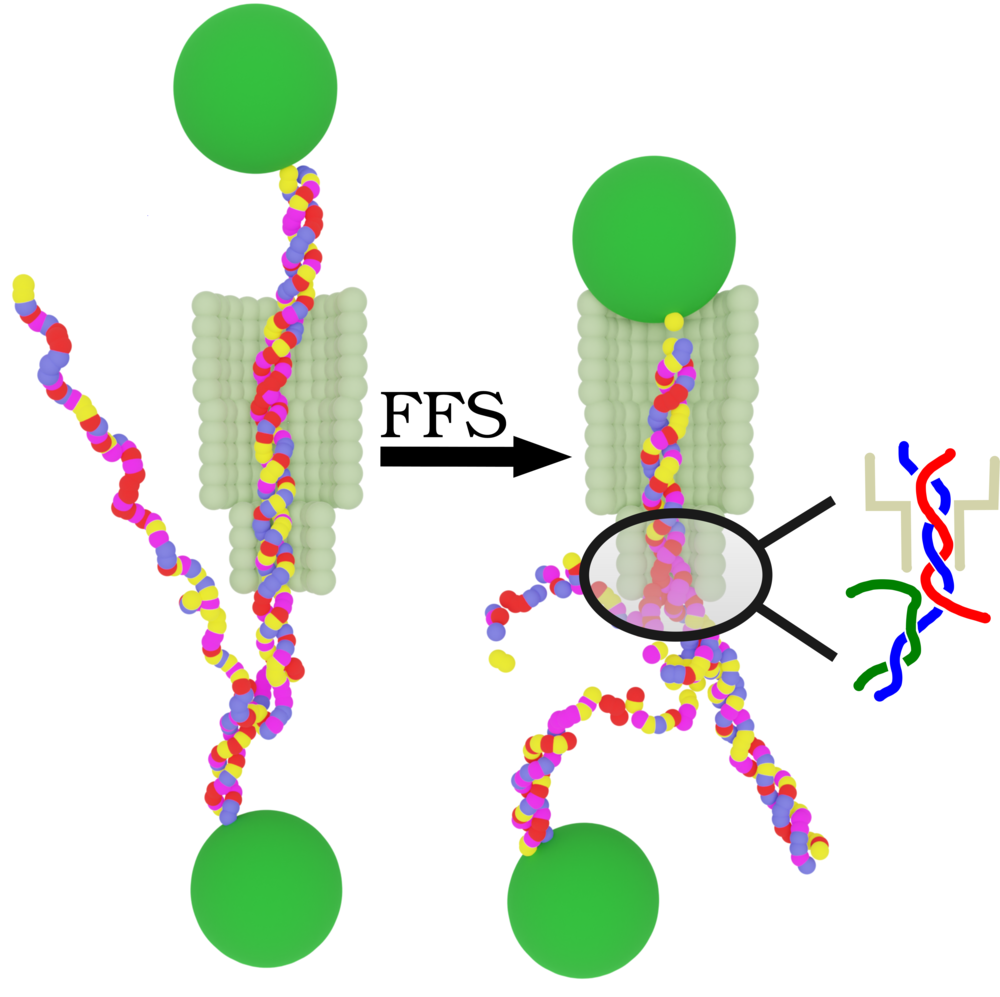
\includegraphics[width=0.7\linewidth]{Figures/hybridisation.png}
  \caption[Simulation result of strand displacement reaction.]{{\small On the left,
        initial configuration of the strand displacement reaction, simulated using the
        Forward Flux Sampling (FFS) method.  On the right, the end state of the
        simulation with the three ssDNA strands entering the pore entrance.
        The problamatic region of the simulation is highlighted and enlarged using an
        illustration, clearifying the limitation of our coarse-grained model. Images
  rendered using Blender.\cite{blender}}}
\end{figure}

